\begin{homeworkProblem}

\textbf{Three Server Organizations}: in the following figure, we show three data center systems with the same arriving rate $\lambda$ and the same total service rate $k \mu$ : FDM, M/M/1 and M/M/k. Please discuss the pros and cons of each system. Regarding the performance of average delay, which system is the best? Show your analysis (CTMC \& Queueing Theory) and simulation results.

\begin{figure}[h]
    \centering
    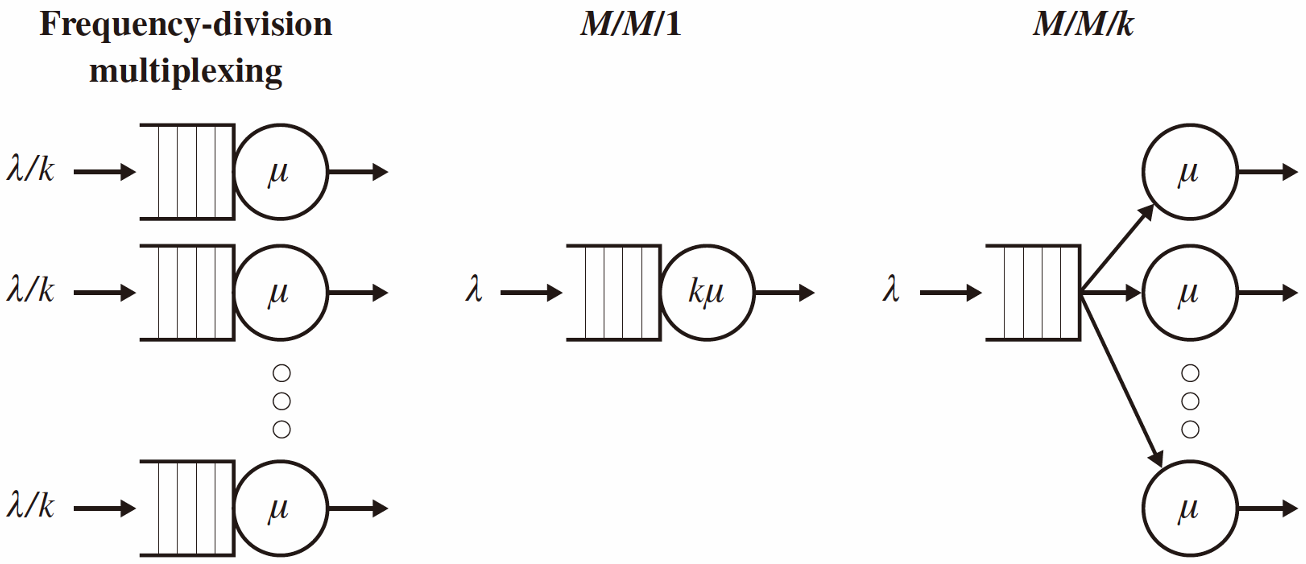
\includegraphics[width=0.7\textwidth]{./figure/servers.png}
\end{figure}

\solution

\textbf{To ensure the total system is stable, the arrival rate should be less than the  service rate, i.e.} $$\lambda < \mu$$
Intuitive understanding is that if the survice rate is less than the arrival rate, which means that the average survice time is less than the average arrival interval, then the system will continously queueing.

\textcolor{blue}{The numertical results for the systems' average delay:} \\
1. M/M/1: the number of customers in the system could be modeled as the following CTMC:
\begin{center}
\begin{tikzpicture}[->, >=stealth, auto, thick, node distance=2cm]
    \tikzstyle{every state} = [
        fill=blue!20,
        draw=black,
        circle,
        minimum size=30pt,
        font=\large\bfseries
    ]

    \node[state] (1) at (-6, 0) {0};
    \node[state] (2) at (-4,  0) {1};
    \node[state] (3) at (-2,  0) {2};
    \node[state, draw=none, fill=none] (ellipsis1) at (0,0) {$\cdots$};
    \node[state] (4) at (2,  0) {$i$};
    \node[state] (5) at (4,  0) {$i+1$};
    \node[state, draw=none, fill=none] (ellipsis2) at (6,0) {$\cdots$};

    \path (1) edge[bend left=30] node{$\lambda$} (2);
    \path (2) edge[bend left=30] node{$k\mu$} (1);
    \path (2) edge[bend left=30] node{$\lambda$} (3);
    \path (3) edge[bend left=30] node{$k\mu$} (2);
    \path (3) edge[bend left=30] node{$\lambda$} (ellipsis1);
    \path (ellipsis1) edge[bend left=30] node{$k\mu$} (3);
    \path (ellipsis1) edge[bend left=30] node{$\lambda$} (4);
    \path (4) edge[bend left=30] node{$k\mu$} (ellipsis1);
    \path (4) edge[bend left=30] node{$\lambda$} (5);
    \path (5) edge[bend left=30] node{$k\mu$} (4);
    \path (5) edge[bend left=30] node{$\lambda$} (ellipsis2);
    \path (ellipsis2) edge[bend left=30] node{$k\mu$} (5);
\end{tikzpicture}
\end{center}

Let $\bpi$ be the stationary distribution of the above CTMC, then according to the detailed balance equation, we have:
$$\pi_i\cdot\lambda = \pi_{i+1}\cdot(k\mu), \forall i\geq 0$$
i.e. $\pi_{i+1} = \dfrac{\lambda}{k\mu}\pi_i\Rightarrow \pi_i = \left(\dfrac{\lambda}{k\mu}\right)^i\pi_0$. \\
And since $\bpi$ is a probability distribution, we have:
$$\sum_{i=0}^{\infty}\pi_i = 1\Rightarrow \pi_0\sum_{i=0}^{\infty}\left(\dfrac{\lambda}{k\mu}\right)^i = 1\Rightarrow \pi_0 = \dfrac{1}{\sum\limits_{i=0}^{\infty}\left(\dfrac{\lambda}{k\mu}\right)^i} = \dfrac{1}{\dfrac{1}{1-\dfrac{\lambda}{k\mu}}}=1-\dfrac{\lambda}{k\mu}$$
Thus, we have
$$\pi_i=\left(1-\dfrac{\lambda}{k\mu}\right)\left(\dfrac{\lambda}{k\mu}\right)^i$$
The average number of customers $L$ in the system is
$$L=\sum_{i=0}^{\infty}i\cdot\pi_i = \dfrac{\left(1-\dfrac{\lambda}{k\mu}\right)\dfrac{\lambda}{k\mu}}{\left(1-\dfrac{\lambda}{k\mu}\right)^2}=\dfrac{\lambda}{k\mu-\lambda}$$
According to the Little's Law, the average delay $W$ is
$$L=\lambda W\Rightarrow W=\dfrac{L}{\lambda}=\dfrac{1}{k\mu-\lambda}$$

2. Frequncy-division multiplexing (FDM): \\
Each server could be regard as a M/M/1 system, but the arriving rate is transformed to $\dfrac{\lambda}{k}$, and the service rate is transformed to $\dfrac{k\mu}{k}=\mu$.  and the average delay is
$$W=\dfrac{k\cdot \frac{1}{\mu-\frac{\lambda}{k}}}{k}=\dfrac{1}{\mu-\frac{\lambda}{k}}$$

3. M/M/k: the number of customers in the system could be modeled as the following CTMC:
\begin{center}
\begin{tikzpicture}[->, >=stealth, auto, thick, node distance=2cm]
    \tikzstyle{every state} = [
        fill=blue!20,
        draw=black,
        circle,
        minimum size=30pt,
        font=\large\bfseries
    ]

    \node[state] (1) at (-6, 0) {0};
    \node[state] (2) at (-4,  0) {1};
    \node[state] (3) at (-2,  0) {2};
    \node[state, draw=none, fill=none] (ellipsis1) at (0,0) {$\cdots$};
    \node[state] (4) at (2,0) {$i$};
    \node[state, draw=none, fill=none] (ellipsis2) at (4,0) {$\cdots$};
    \node[state] (5) at (6,  0) {$k$};
    \node[state] (6) at (8,  0) {$k$+1};
    \node[state, draw=none, fill=none] (ellipsis3) at (10,0) {$\cdots$};

    \path (1) edge[bend left=30] node{$\lambda$} (2);
    \path (2) edge[bend left=30] node{$\mu$} (1);
    \path (2) edge[bend left=30] node{$\lambda$} (3);
    \path (3) edge[bend left=30] node{$2\mu$} (2);
    \path (3) edge[bend left=30] node{$\lambda$} (ellipsis1);
    \path (ellipsis1) edge[bend left=30] node{$3\mu$} (3);
    \path (ellipsis1) edge[bend left=30] node{$\lambda$} (4);
    \path (4) edge[bend left=30] node{$i\mu$} (ellipsis1);
    \path (4) edge[bend left=30] node{$\lambda$} (ellipsis2);
    \path (ellipsis2) edge[bend left=30] node{$(i+1)\mu$} (4);
    \path (ellipsis2) edge[bend left=30] node{$\lambda$} (5);
    \path (5) edge[bend left=30] node{$k\mu$} (ellipsis2);
    \path (5) edge[bend left=30] node{$\lambda$} (6);
    \path (6) edge[bend left=30] node{$k\mu$} (5);
    \path (6) edge[bend left=30] node{$\lambda$} (ellipsis3);
    \path (ellipsis3) edge[bend left=30] node{$k\mu$} (6);
\end{tikzpicture}
\end{center}
Let $T_i$ be the survice time of the $i$-th server, i.e. $T_i\sim \Expo(\mu)$. Since we have known that
$$\min\left(\Expo(\lambda_1),\ldots,\Expo(\lambda_n)\right)\sim\Expo(\lambda_1+\ldots+\lambda_n)$$
So when $t$ servers are working, the time of the next server to be idle is
$$T=\min\left(T_1,\ldots,T_t\right)\sim\Expo(t\mu)$$
Thus the death rate when $t$ servers are working is $t\mu$. So the above CTMC is a birth-death process with parameter shown in the chain. \\
Let $\bpi$ be the stationary distribution of the above CTMC, then according to the detailed balance equation, we have:
\begin{align*}
\pi_i\cdot\lambda &= \pi_{i+1}\cdot((i+1)\mu), \forall i\leq k-1 \\
\pi_i\cdot\lambda &= \pi_{i+1}\cdot(k\mu) \qquad\ , \forall i\geq k
\end{align*}
Thus, we can express $\pi_i$ with $\pi_0$ as:
\begin{align*}
\pi_i &= \dfrac{\lambda}{i\mu}\pi_{i-1} = \dfrac{1}{i!}\left(\dfrac{\lambda}{\mu}\right)^i\pi_0 \quad\ , \forall 1\leq i\leq k-1 \\
\pi_i &= \dfrac{\lambda}{k\mu}\pi_{i-1} = \dfrac{k^k}{k!}\left(\dfrac{\lambda}{k\mu}\right)^i\pi_0, \forall i\geq k
\end{align*}
And since $\bpi$ is a probability distribution, we have:
$$\sum_{i=0}^{\infty}\pi_i = 1\Rightarrow \pi_0 = \left[
\left(\sum_{i=0}^{k-1}\dfrac{1}{i!}\left(\dfrac{\lambda}{\mu}\right)^i\right)+
\dfrac{1}{k!}\left(\dfrac{\lambda}{\mu}\right)^k\dfrac{1}{1-\frac{\lambda}{k\mu}}\right]^{-1}$$

Since if there are less or equal to $k$ customers, they would never be in the queue, but just use the survice for the survices, so the average number of customers $L_q$ in the queue is
\begin{align*}
L_q &= \sum_{i=k+1}^{\infty}(i-k)\cdot\pi_i \\
&= \sum_{i=k+1}^{\infty}(i-k)\cdot\dfrac{k^k}{k!}\left(\dfrac{\lambda}{k\mu}\right)^i\pi_0
\end{align*}
\begin{align*}
&\stackrel{n=i-k}{=} \left(\dfrac{\lambda}{k\mu}\right)^k\dfrac{k^k\pi_0}{k!}\sum_{n=1}^{\infty}n\left(\dfrac{\lambda}{k\mu}\right)^n \\
&= \left(\dfrac{\lambda}{\mu}\right)^k\dfrac{\pi_0}{k!}\dfrac{\frac{\lambda}{k\mu}}{(1-\frac{\lambda}{k\mu})^2}
\end{align*}
According to the Little's Law, the average time the customers are in the queue $W_q$ is
$$L_q=\lambda W_q\Rightarrow W_q=\dfrac{L_q}{\lambda} = \left(\dfrac{\lambda}{\mu}\right)^k\dfrac{\pi_0}{(k!)(k\mu)(1-\frac{\lambda}{k\mu})^2}$$
Where
$$\pi_0 = \left[\left(\sum_{i=0}^{k-1}\dfrac{1}{i!}\left(\dfrac{\lambda}{\mu}\right)^i\right)+\dfrac{1}{k!}\left(\dfrac{\lambda}{\mu}\right)^k\dfrac{1}{1-\frac{\lambda}{k\mu}}\right]^{-1}$$
Since the surver's service rate is $\mu$, i.e. the survice time is $\Expo(\mu)$, so the average time customers spend in the surver is $\dfrac{1}{\mu}$, so the average delay $W$ is
$$W=W_q+\dfrac{1}{\mu}= \left(\dfrac{\lambda}{\mu}\right)^k\dfrac{\pi_0}{(k!)(k\mu)(1-\frac{\lambda}{k\mu})^2}+\dfrac{1}{\mu}$$

\textcolor{blue}{The performance comparison of the systems:} \\
Define $\rho=\dfrac{\lambda}{\mu}$. As mentioned in the beginning, we have $\lambda<\mu\Rightarrow \rho\in(0,1)$. \\
1. Prove $W_{\text{M/M/1}} \leq W_{\text{M/M/k}}$, the following steps are what we need to prove:
\begin{align*}
\dfrac{1}{k\mu-\lambda} &\leq \dfrac{1}{\mu} + \rho^k\dfrac{1}{(k!)(k\mu)\left(1-\frac{\rho}{k}\right)^2}\dfrac{1}{\pi_0} \\
\dfrac{\lambda-(k-1)\mu}{(k\mu-\lambda)\mu}\cdot\pi_0 &\leq \dfrac{\rho^k}{(k!)(k\mu)\left(1-\frac{\rho}{k}\right)^2} \\
\left(\sum_{i=0}^{k-1}\dfrac{\rho^i}{i!}\right)+\dfrac{1}{k!}\dfrac{\rho^k}{1-\frac{\rho}{k}} &\leq \dfrac{\rho^k\cdot (k\mu-\lambda)}{k(k!)\left(1-\frac{\rho}{k}\right)^2\left[\lambda-(k-1)\mu\right]} \\
\sum_{i=0}^{k-1}\dfrac{\rho^i}{i!} &\leq \dfrac{\rho^k\cdot \left[k^2\mu+(2k-\rho)\lambda\right]}{k(k!)\left(1-\frac{\rho}{k}\right)^2\left[\lambda-(k-1)\mu\right]}
\end{align*}
When $k=1$, the inequality obviously holds, and the equality holds. \\
Use the deduction, suppose the inequality holds $\forall n=1,2,\ldots,k$, i.e.
$$\sum_{i=0}^{n-1}\dfrac{\rho^i}{i!} \leq \dfrac{\rho^n\cdot \left[n^2\mu+(2n-\rho)\lambda\right]}{n(n!)\left(1-\frac{\rho}{n}\right)^2\left[\lambda-(n-1)\mu\right]}$$
then for $n=k+1$, we only need to prove that
\begin{align*}
\dfrac{\rho^n}{n!} &\leq \dfrac{\rho^{n+1}\cdot \left[(n+1)^2\mu+(2(n+1)-\rho)\lambda\right]}{(n+1)((n+1)!)\left(1-\frac{\rho}{n+1}\right)^2\left[\lambda-((n+1)-1)\mu\right]} - \dfrac{\rho^n\cdot \left[n^2\mu+(2n-\rho)\lambda\right]}{n(n!)\left(1-\frac{\rho}{n}\right)^2\left[\lambda-(n-1)\mu\right]} \\
1 &\leq \dfrac{\rho\cdot \left[(n+1)^2\mu+(2(n+1)-\rho)\lambda\right]}{(n+1)^2\left(1-\frac{\rho}{n+1}\right)^2\left[\lambda-n\mu\right]} - \dfrac{n^2\mu+(2n-\rho)\lambda}{n\left(1-\frac{\rho}{n}\right)^2\left[\lambda-(n-1)\mu\right]}
\end{align*}
Since $\rho\in(0,1)$, so the above inequality holds, thus
$$W_{\text{M/M/1}} \leq W_{\text{M/M/k}}$$

2. Prove $W_{\text{M/M/k}} \leq W_{\text{FDM}}$, we have a similar steps:
\begin{align*}
\dfrac{1}{\mu} + \rho^k\dfrac{1}{(k!)(k\mu)\left(1-\frac{\rho}{k}\right)^2}\dfrac{1}{\pi_0} &\leq \dfrac{1}{\mu-\frac{\lambda}{k}} \\
\sum_{i=0}^{k-1}\dfrac{\rho^i}{i!} &\leq \dfrac{\rho^k\cdot \left[k^2\mu+(2k-\rho)\lambda\right]}{(k!)\left(1-\frac{\rho}{k}\right)^2\left[\lambda-(k-1)\mu\right]}
\end{align*}
It has a similar process, instread that a $k$ is times to the right hand side, thus
$$W_{\text{M/M/k}} \leq W_{\text{FDM}}$$

\textcolor{blue}{So above all, the average delay of the three systems are}
\begin{align*}
W_{\text{FDM}} &= \dfrac{1}{\mu-\frac{\lambda}{k}} \\
W_{\text{M/M/1}} &= \dfrac{1}{k\mu-\lambda} \\
W_{\text{M/M/k}} &= \dfrac{1}{\mu} + \left(\dfrac{\lambda}{\mu}\right)^k\dfrac{1}{(k!)(k\mu)(1-\frac{\lambda}{k\mu})^2}\left[\left(\sum_{i=0}^{k-1}\dfrac{1}{i!}\left(\dfrac{\lambda}{\mu}\right)^i\right)+\dfrac{1}{k!}\left(\dfrac{\lambda}{\mu}\right)^k\dfrac{1}{1-\frac{\lambda}{k\mu}}\right]^{-1}
\end{align*}

And the performance of average delay of the three systems are
$$W_{\text{M/M/1}} \leq W_{\text{M/M/k}} \leq W_{\text{FDM}}$$
If and only if when $k=1$, the equality holds.

\textcolor{blue}{Pros and cons:}
\begin{itemize}
\item FDM: \\
Pros: It is simply implemented and fault-isolated. It would not cause too much trouble if some of the queues or servers have faults. \\
Cons: Its drawbacks include lower resource utilization and load imbalances that can lead to increased latency.

\item M/M/1: \\
Pros: Centralized queuing facilitates optimal resource sharing, which can significantly reduce the average latency. It concentrates efforts to accomplish great things. \\
Cons: It does risk a single point of bottleneck, if the queue or the server has errors, the whole system will collapse.

\item M/M/k: \\
Pros: Parallel servers offer a certain degree of fault tolerance and distributed benefits \\
Cons: Its scheduling efficiency is not as high as that of a centralized system, resulting in an average latency that falls between the other two.
\end{itemize}

Therefore, as long as the system remains stable and the load is moderate, the M/M/1 system is the optimal choice in terms of average latency.

\textcolor{blue}{Simulation results:} \\
The simulation has total $1000000$ customers, with different arrival rate and service rate, and $k$. The details could be seen in hw2\_code.ipynb, theoretical results are also in it, which could be found that the simulated results are quite close to the theoretical results. And $W_q$ represent the avreage waiting time, $W_s$ represent the avreage service time, $W=W_q+W_s$ is the average delay. \\
The simulation with different settings are as followed.
\begin{figure}[h]
    \centering
    Settings: the arrival rate $\lambda = 0.1$, service rate $\mu = 0.15$, and $k=3$.
    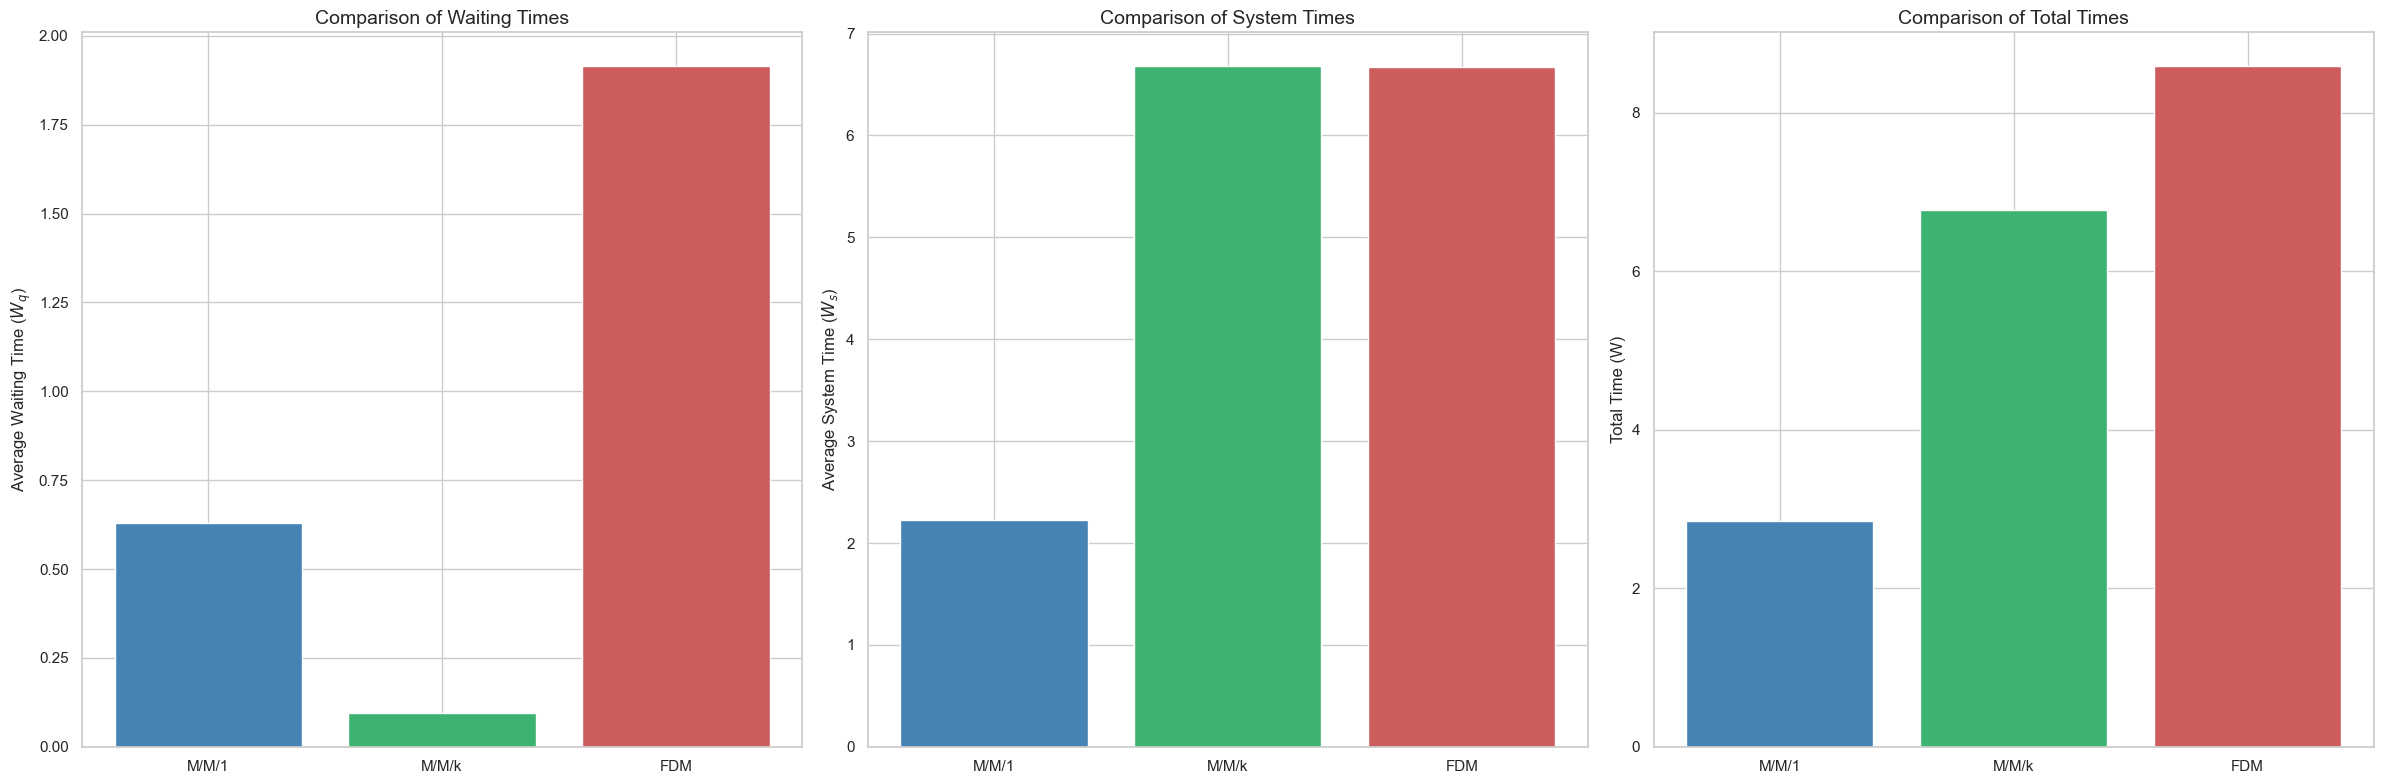
\includegraphics[width=\textwidth]{./figure/scenario1.png}
    Settings: the arrival rate $\lambda = 0.1$, service rate $\mu = 0.15$, and $k=10$.
    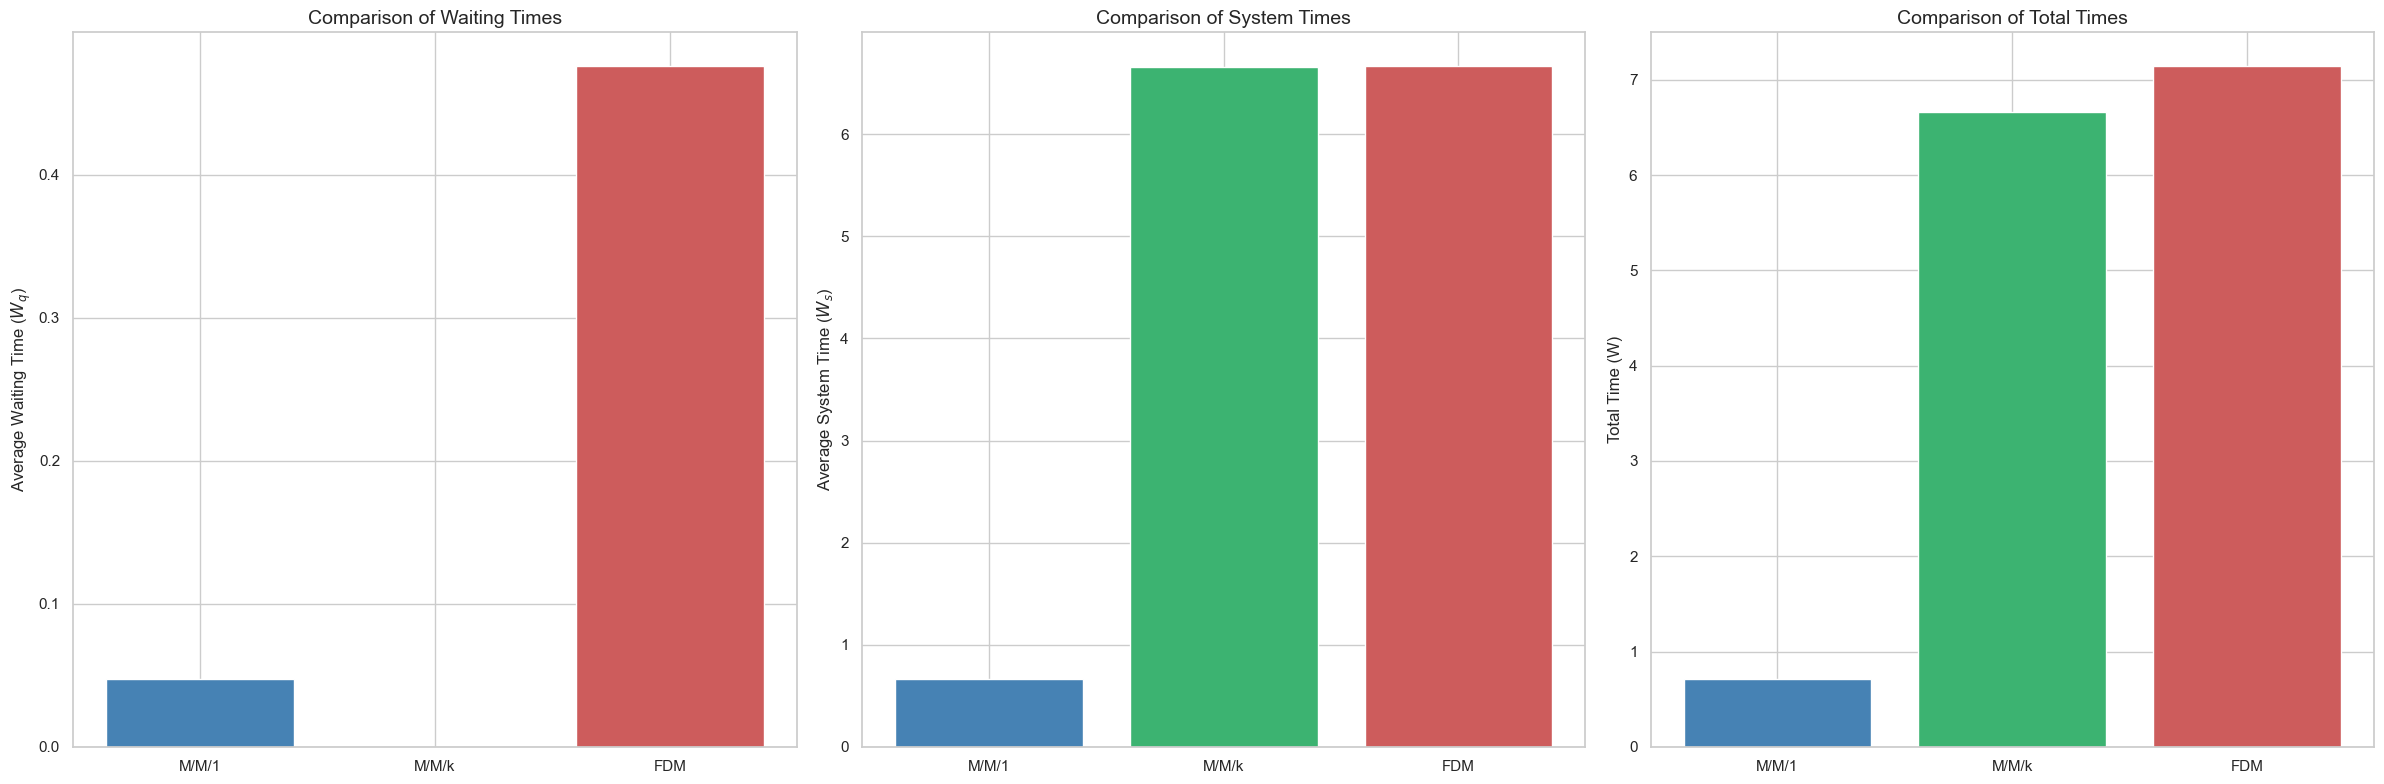
\includegraphics[width=\textwidth]{./figure/scenario2.png}
    Settings: the arrival rate $\lambda = 0.1$, service rate $\mu = 0.2$, and $k=3$.
    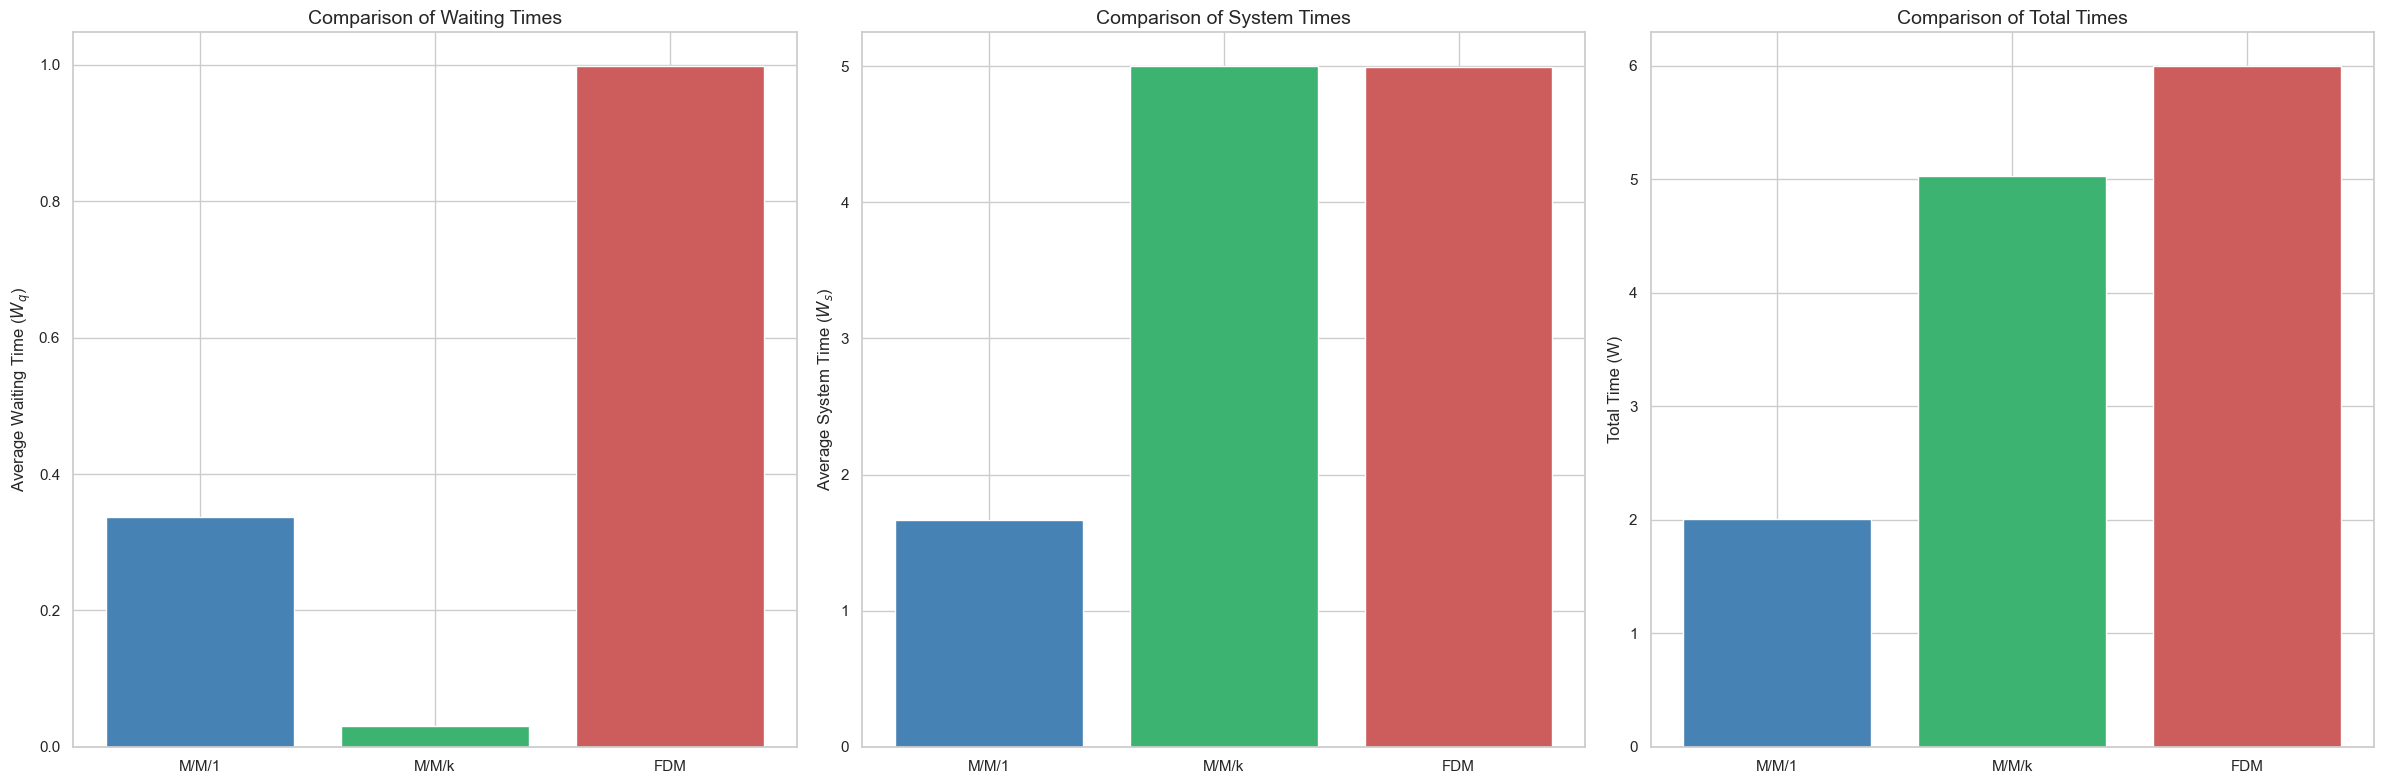
\includegraphics[width=\textwidth]{./figure/scenario3.png}
\end{figure}
\vspace{1.0in}
\begin{figure}[h]
    \centering
    Settings: the arrival rate $\lambda = 0.1$, service rate $\mu = 0.2$, and $k=10$.
    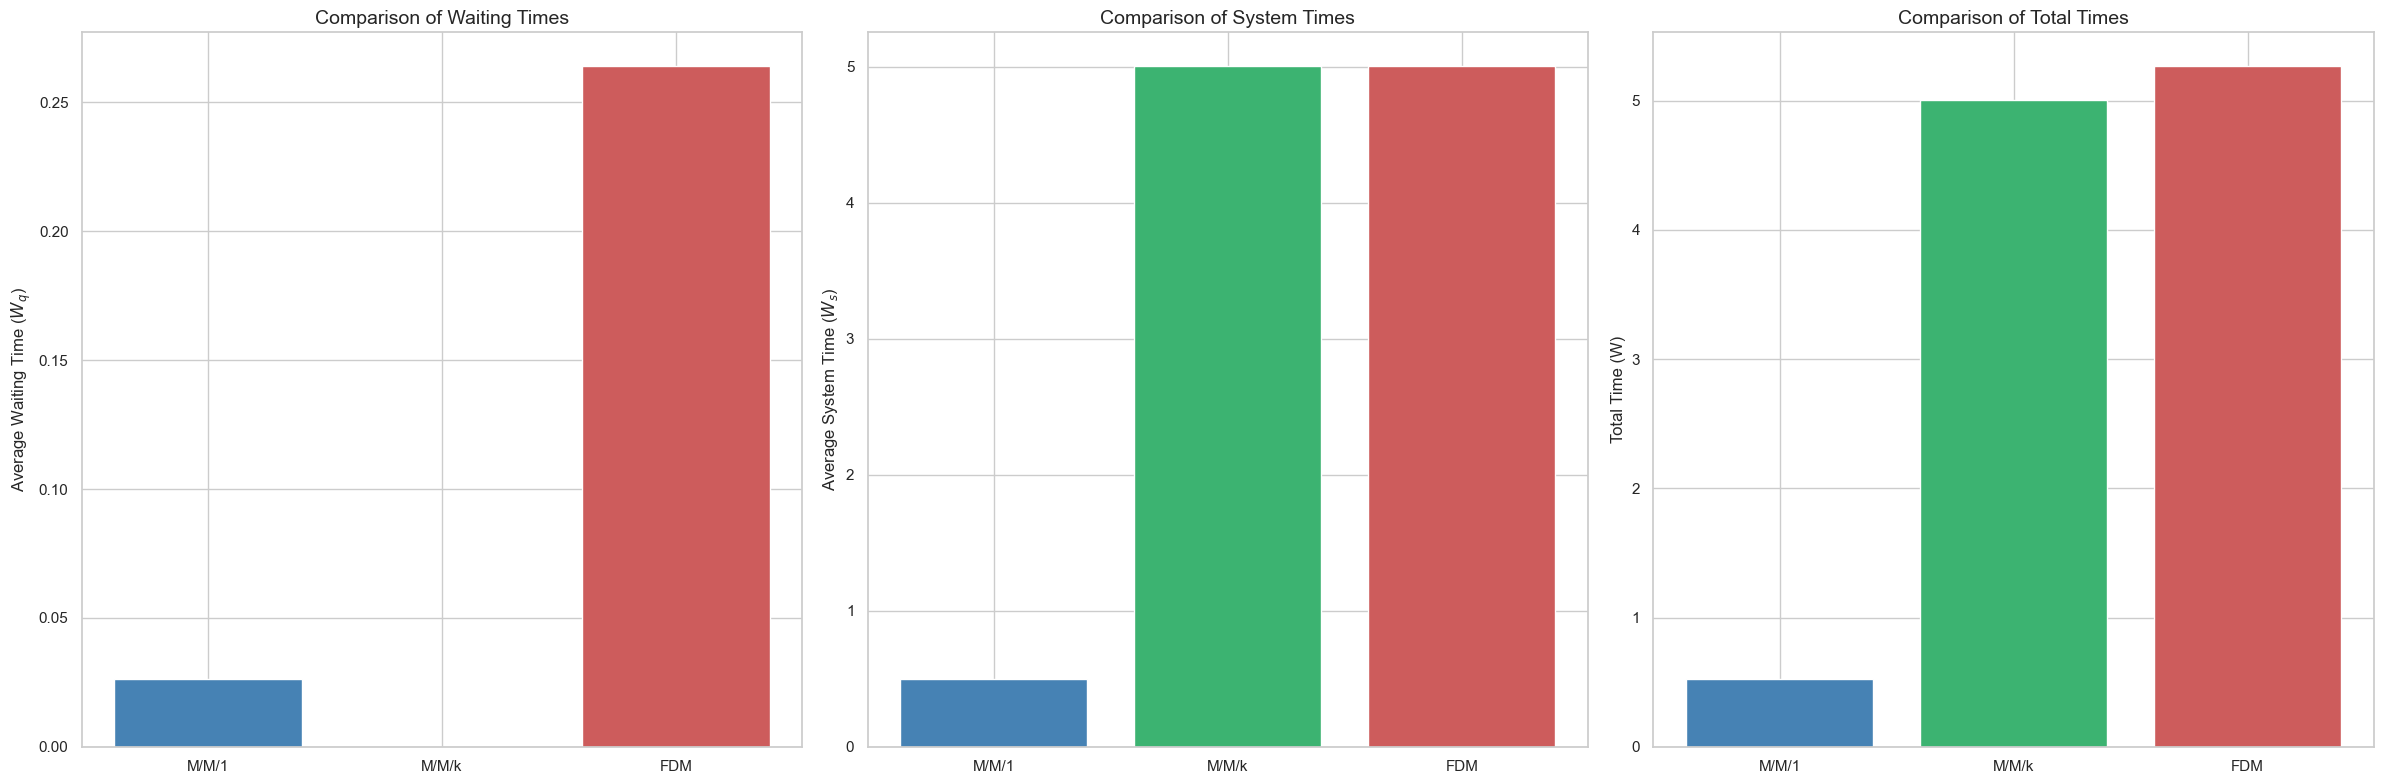
\includegraphics[width=\textwidth]{./figure/scenario4.png}
    Settings: the arrival rate $\lambda = 0.1$, service rate $\mu = 1.0$, and $k=3$.
    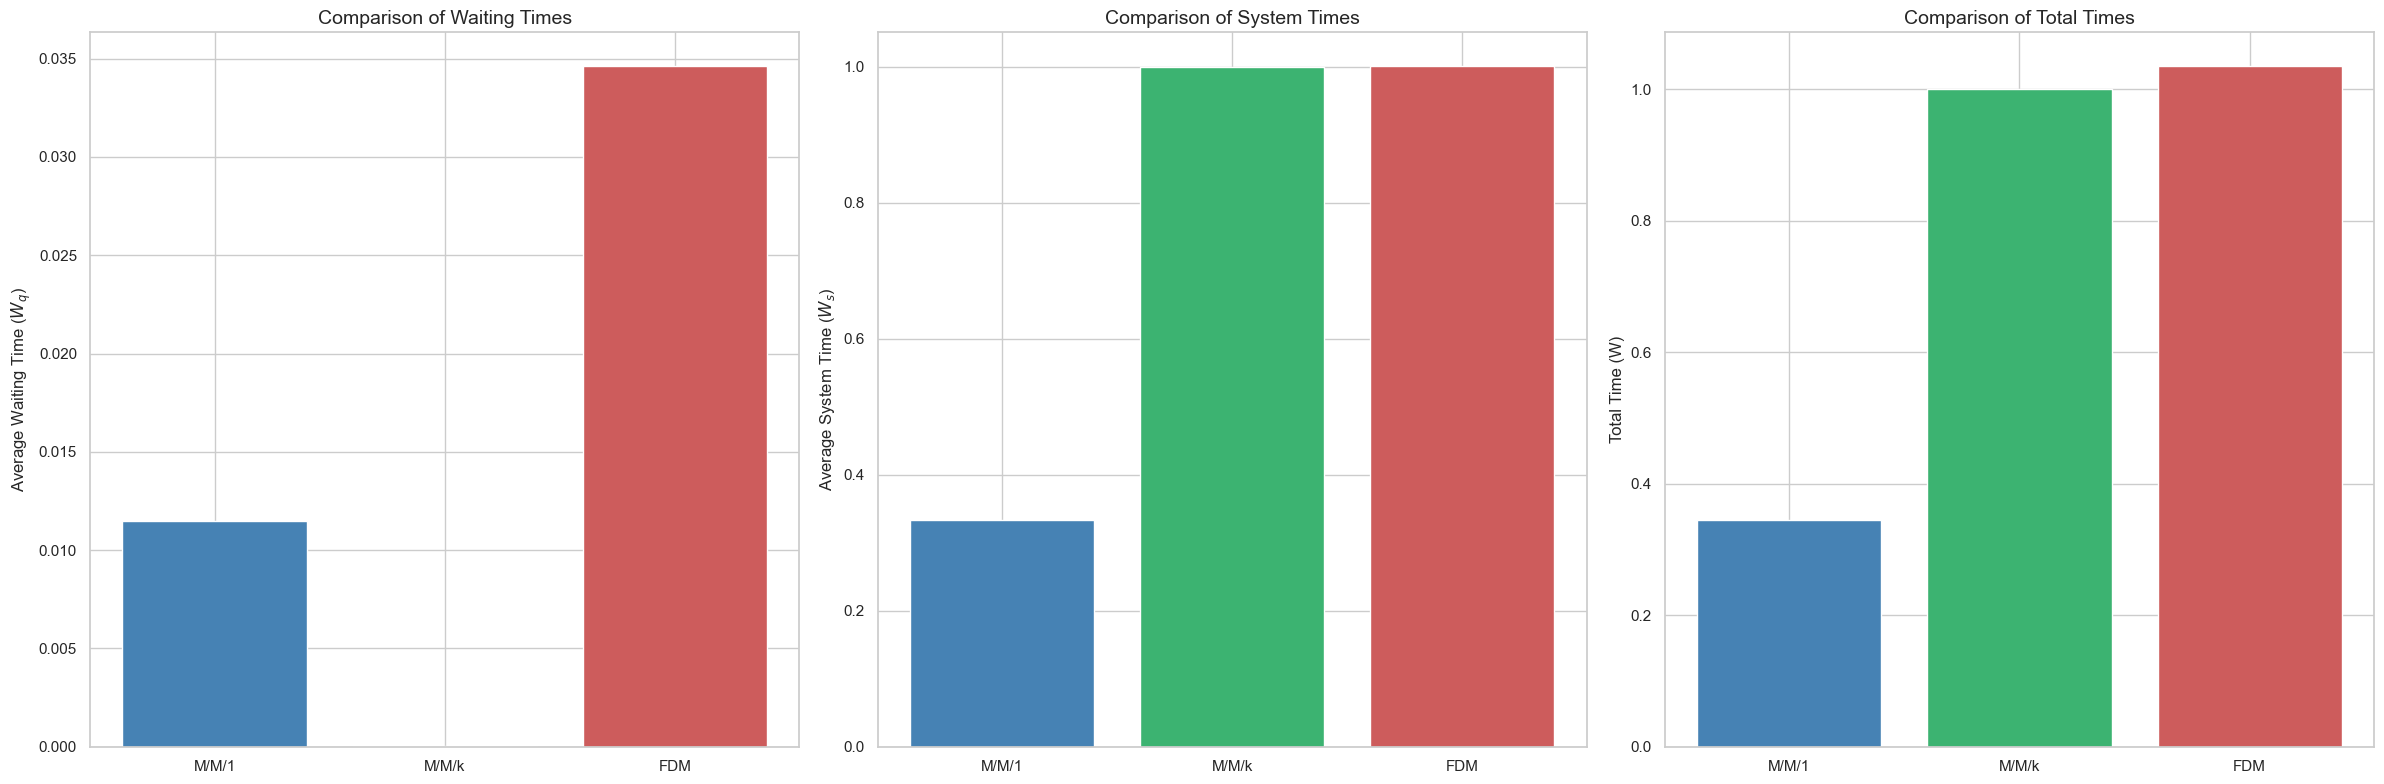
\includegraphics[width=\textwidth]{./figure/scenario5.png}
    Settings: the arrival rate $\lambda = 0.1$, service rate $\mu = 1.0$, and $k=10$.
    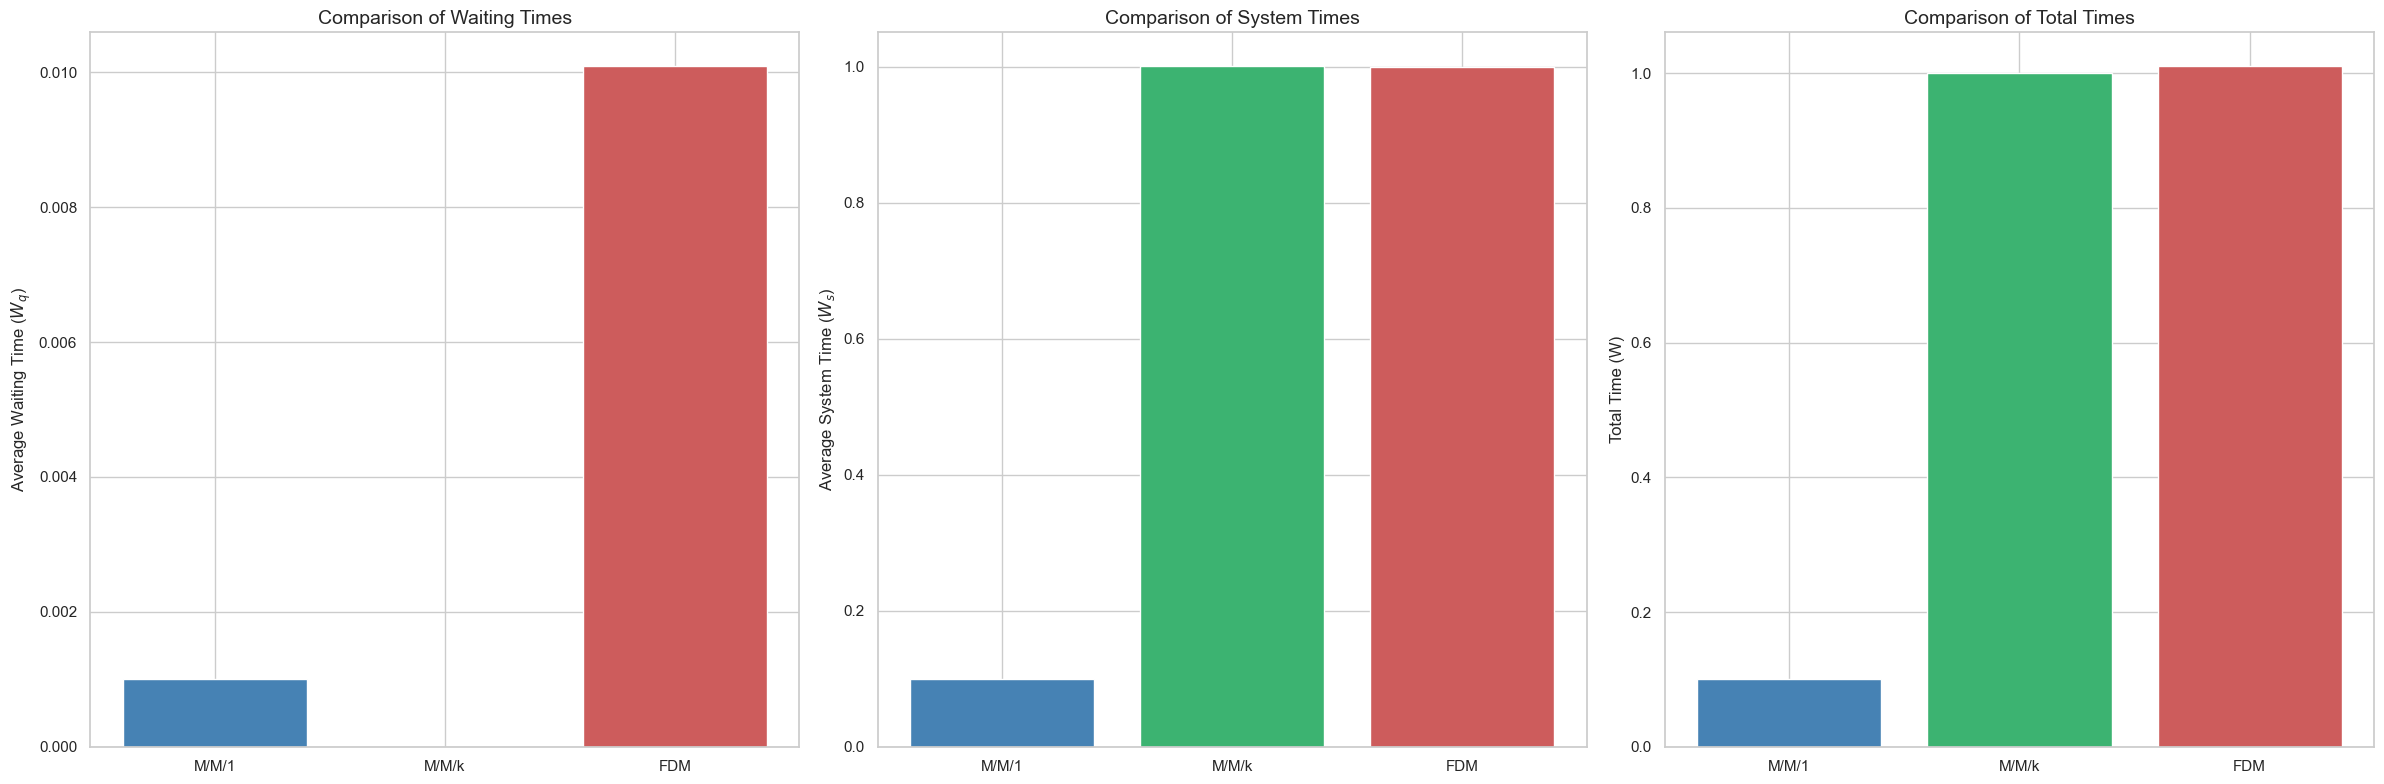
\includegraphics[width=\textwidth]{./figure/scenario6.png}
\end{figure}

From the results, we could see that the average waiting time $W_q$ has M/M/k < M/M/1 < FDM, and the average survice time $W_s$ has M/M/1 < M/M/k = FDM. The average delay $W$ has M/M/1 < M/M/k < FDM. Which fits the theoretical results. The bigger $k$ is, the advantage of M/M/1 on average time delay is more obvious. And the larger $\dfrac{\mu}{\lambda}$ is, the M/M/k is more similar to FDM, while M/M/1 seens to have a much better performance.

\end{homeworkProblem}

\newpage